\documentclass{article}
\usepackage[utf8]{inputenc}
\usepackage[english]{babel}
\usepackage{amsthm}
\usepackage{amssymb}
\usepackage{graphicx}
\graphicspath{ {images/} }
\usepackage{titlesec}
\newcommand{\sectionbreak}{\clearpage}
\usepackage{subcaption}

\author{Kevin Martin\\ CIS657 Monday @ 10:00pm EST\\ Syracuse University}
\title{Lab 1}

\newtheorem{theorem}{Question}
\begin{document}
\maketitle
\section{Introduction}
Before I begin, I would like to state that I did not follow the recommended installation instructions.\\\\
I am running Linux on my home computer, a distribution called Arch. It is a somewhat "minimalist" version, 
and while popular, is not one of the major distributions. As such, I wanted to make sure I could at least get Xinu up and running, 
so I downloaded and configured before the first lives session.\\\\
I used the VirtualBox version that is in the Arch User Repository (AUR), which happens to be version 6.1.0-1. The
recommended method of installation for Arch programs is having a package manager take care of everything from the AUR.\\\\
I am using the correct version of Xinu, from the shared Google Drive link. Other than my version of VirtualBox, the guide and
assignment worked as intended. As such, I believe that there shouldn't be any issues going forward with this project, but 
I understand there exists the potential for complications because of this.

\section{Configuration}
I followed the instructions from Lab 1, and was able to untar the 
xinu-x86-vim.tar.gz and compile the Xinu kernel using the make commmand:\\
\begin{figure}[ht!]
  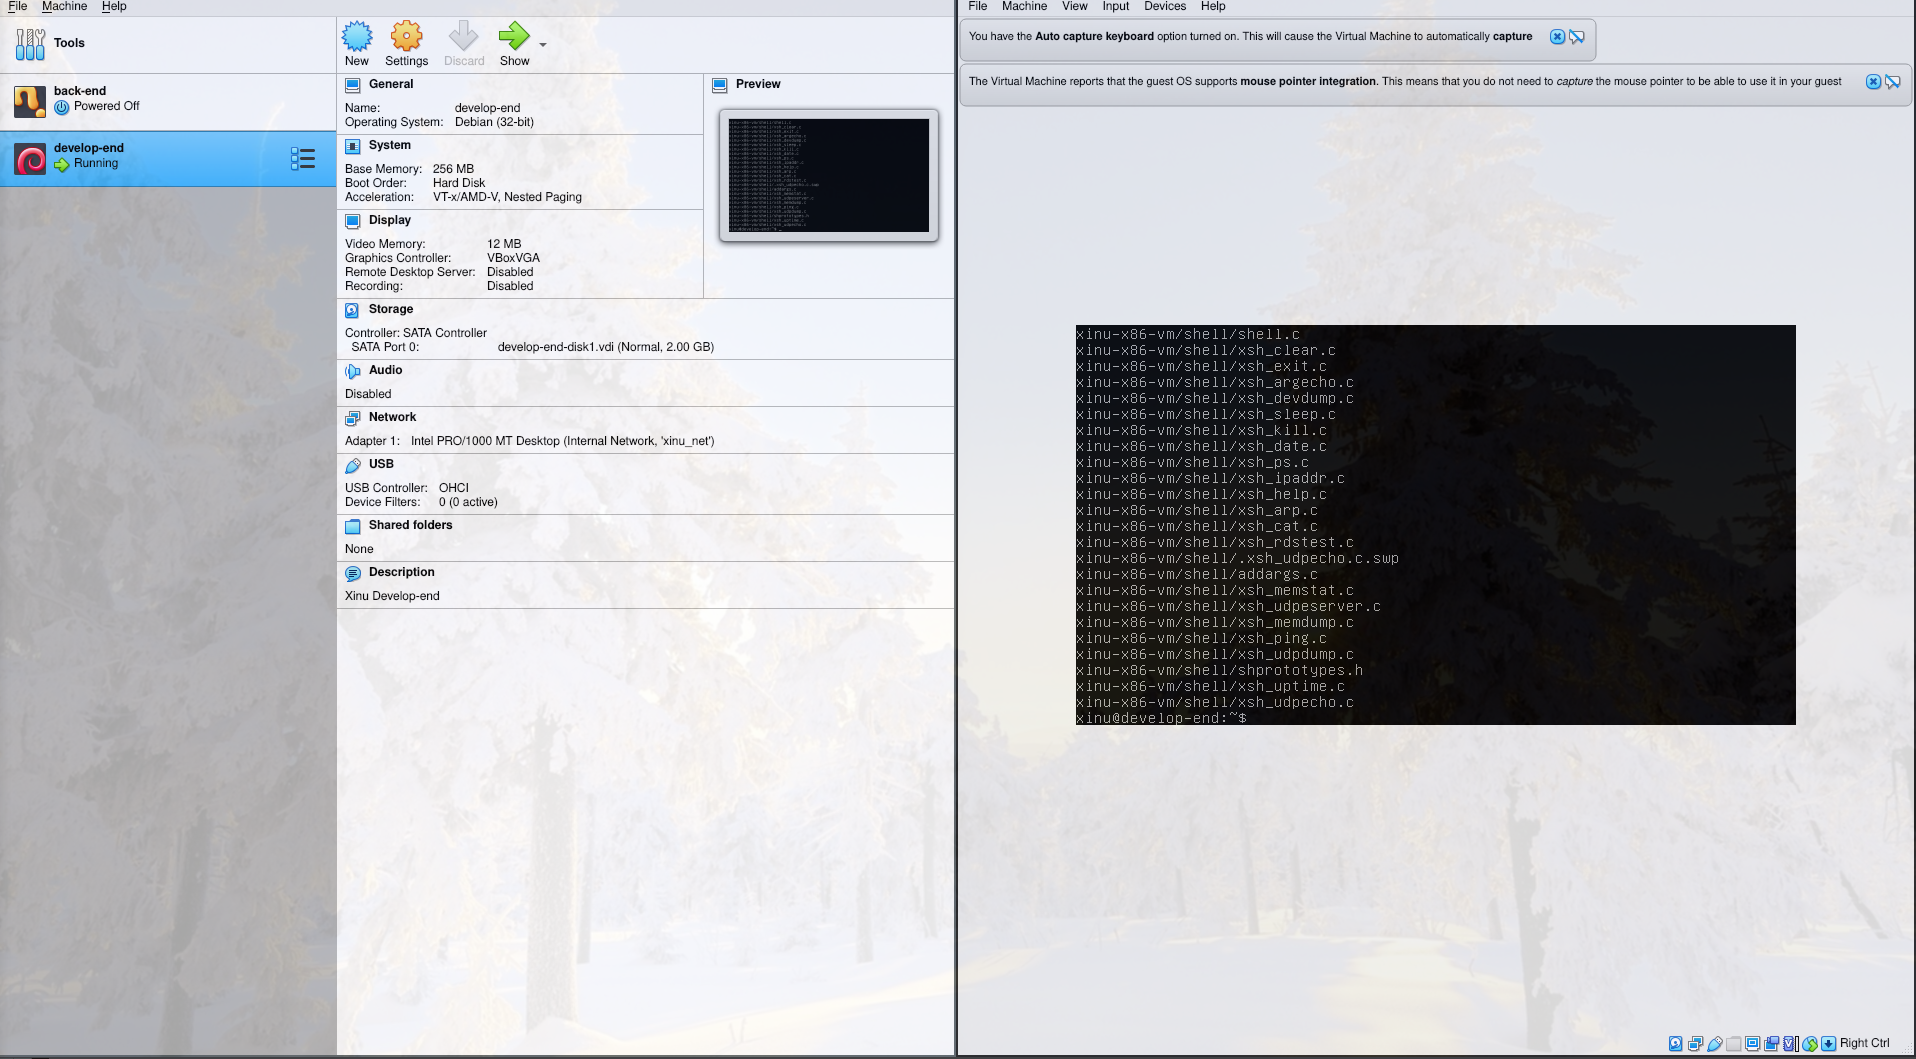
\includegraphics[width=\textwidth]{tar.png}
  \caption{Successful untaring.}
\end{figure}
\begin{figure}[ht!]
  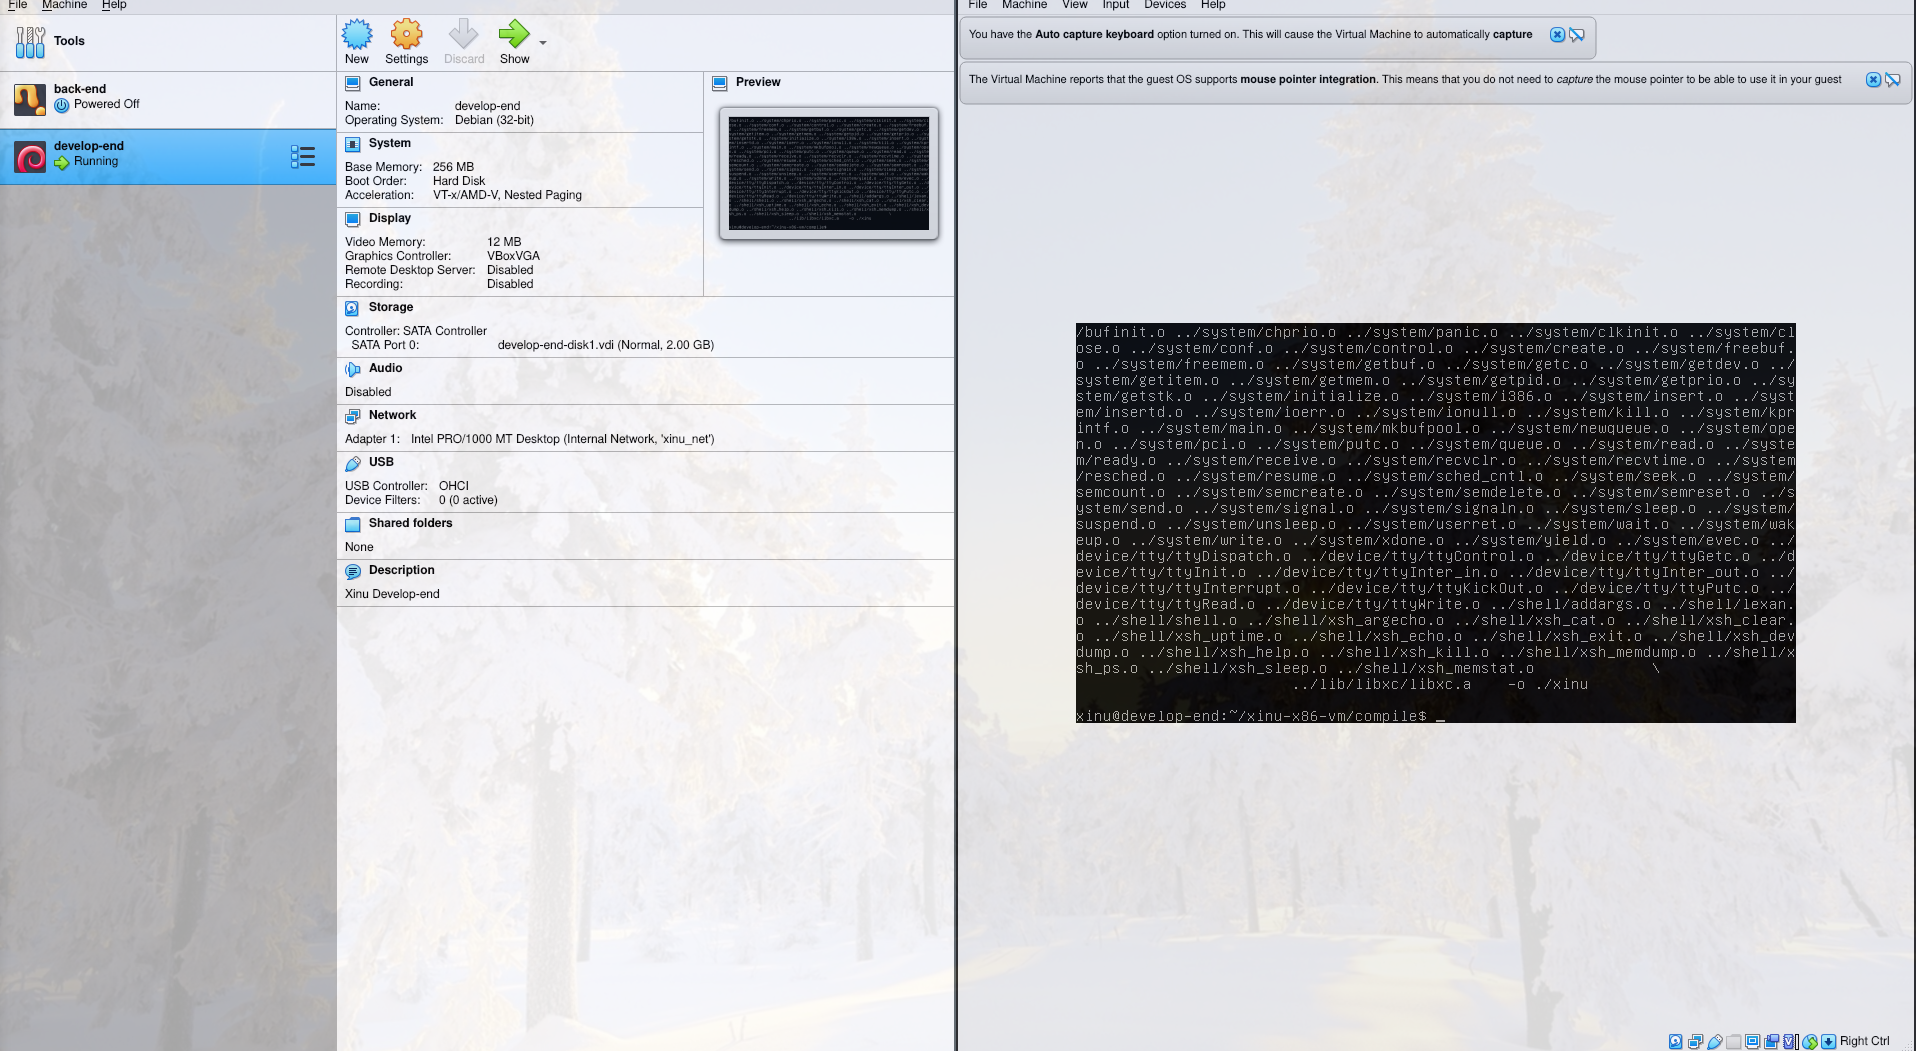
\includegraphics[width=\textwidth]{compile.png}
  \caption{Successful compilation.}
\end{figure}

Finally, I was able to issue "sudo minicom", turn on the back-end machine, and display the big Xinu logo:
\begin{figure}[ht!]
  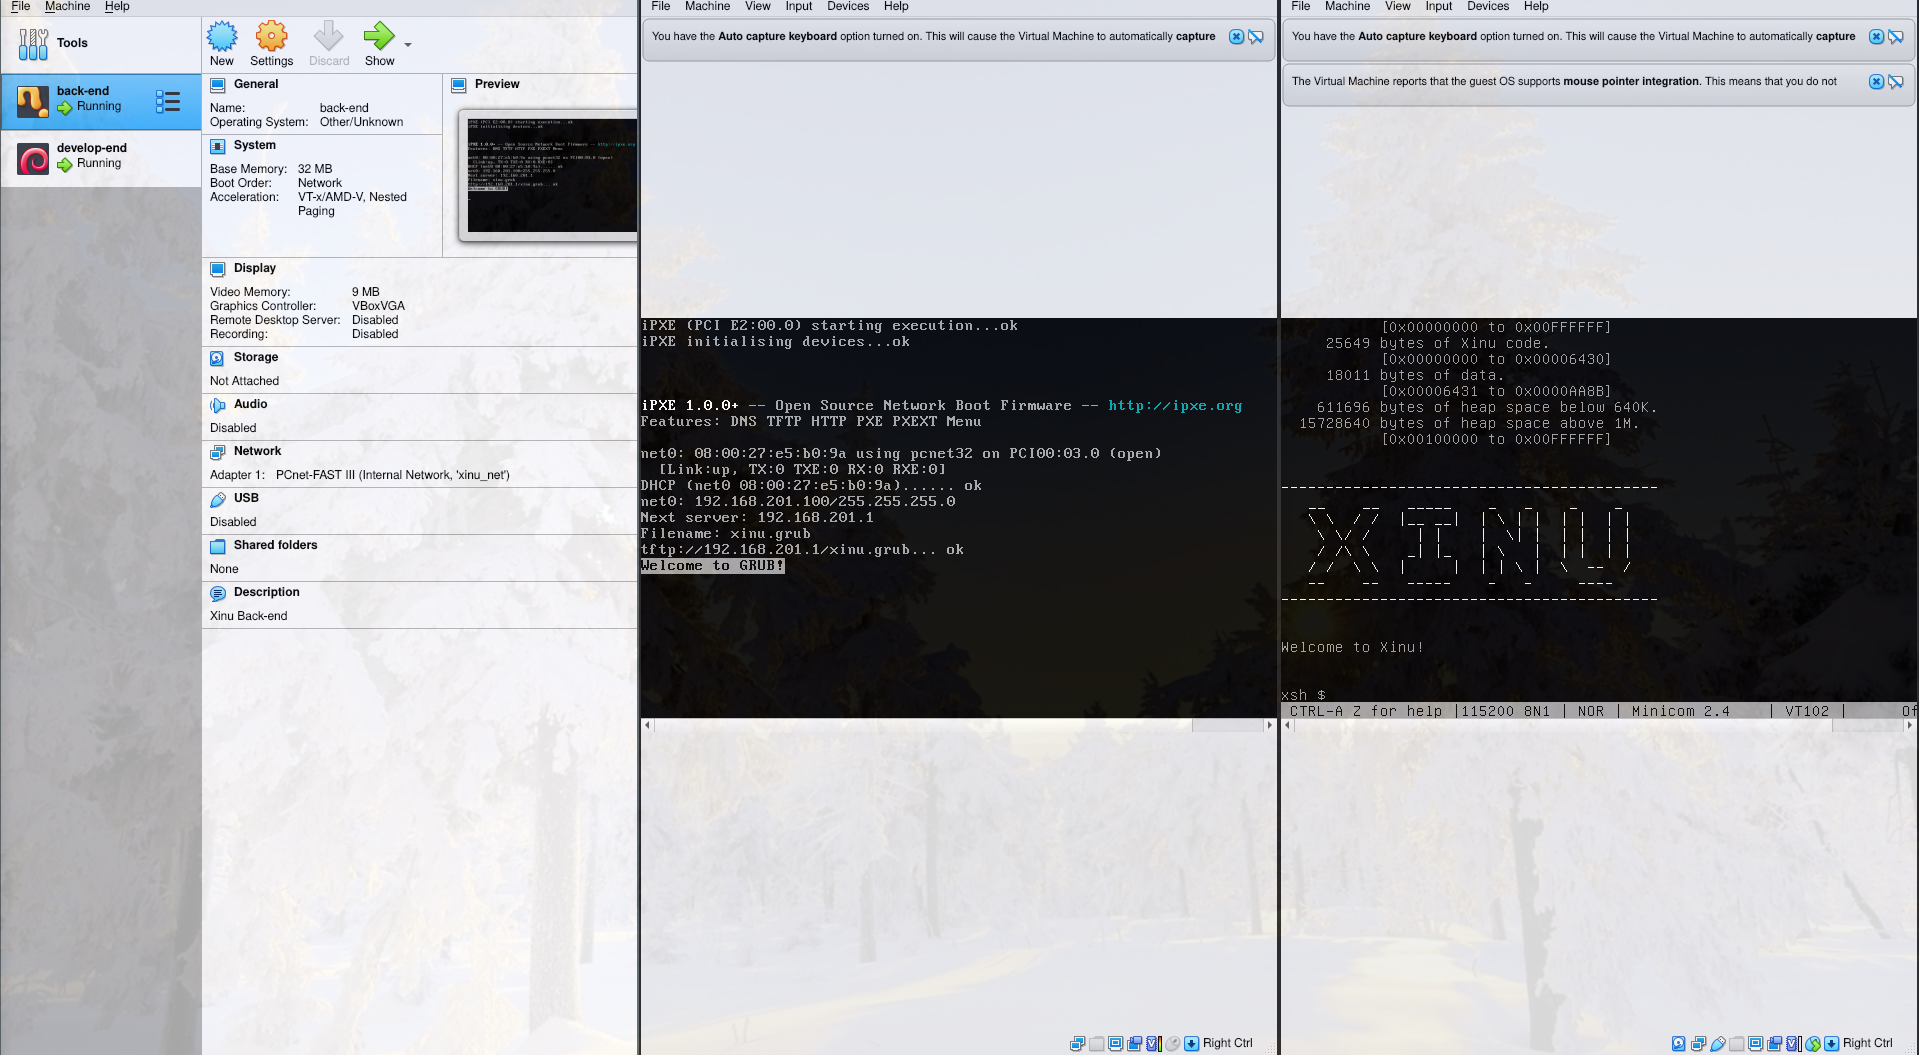
\includegraphics[width=\textwidth]{xinupage.png}
  \caption{Xinu rocks!}
\end{figure}

\section{Part I}
After exiting the minicom, I was able to navigate around the file system using the familiar Linux commands. \\\\
Following the directions, I auto-mounted a folder from my host computer to a newly created "shared" folder. I copied
"main.c" with the command "cp" to make sure I could see it in both places:

\begin{figure}[ht!]
  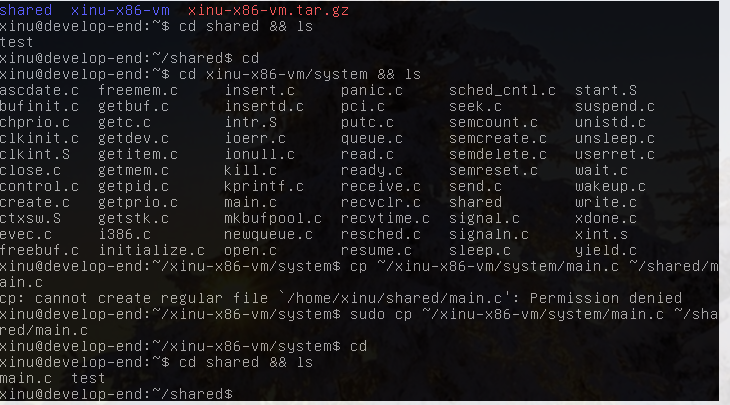
\includegraphics[width=\textwidth]{mainshare.png}
  \caption{Main.c present in the shared directory.}
\end{figure}



\section{Part II}

To investige the files "main.c" and "queue.c", I used the text editor Vi, which came shipped with the Xinu (Linux) kernel.
I use Vim as my text editor for C/C++ files, and recently LaTex. \footnote{This entire homework assignment has been written
in Vim using a LaTex plugin. The two work great together!} This made navigation very familiar:
\begin{figure}[ht!]
  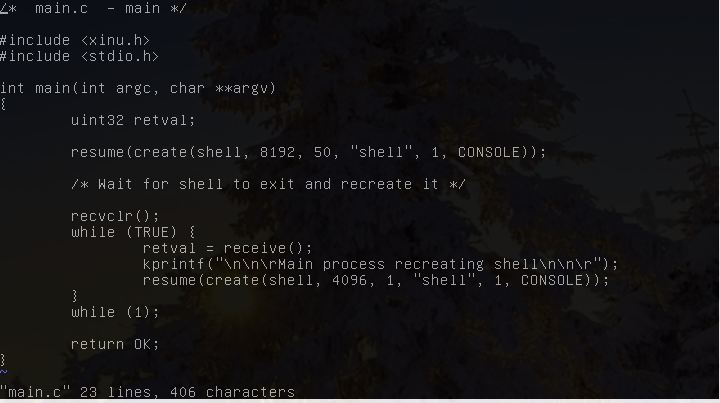
\includegraphics[width=\textwidth]{mainvi.png}
  \caption{Main.c, opened with Vi inside Xinu.}
\end{figure}

\begin{theorem}
While looking through "main.c", it appears to simply create a terminal, using the resume/create process. This makes sense
as on startup, all the user would have access to or need would be a terminal.\\
On inspection of "queue.c", it appears to provide the framework for working with the queue table (queuetab). Apart from simple
 "enqueue" and "dequeue" processes, the functions provide checks to make sure only valid process IDs are added or removed.
The functions also take care of the pointers, ensuring that a new process will point to the correct node, and, similarly,
a process being removed will not break the chain of pointers.
\end{theorem}

\begin{theorem}
The Linux command that enabled me to copy the "xinu-x86-vm" directory to the "shared" directory is:\\\\
sudo cp -r {\textasciitilde{}}/xinu-x86-vm {\textasciitilde{}}/shared\\\\
"Sudo" as the user xinu is apparently not the administrator, "cp" to copy, the modifier "-r" for "recursive" which includes
all the sub-directories and contents, "{\textasciitilde{}}" specifying the root directory starting point,
 the first statement after the modifier is the item to copy, and the second is the destination.\\
\begin{figure}[ht!]
  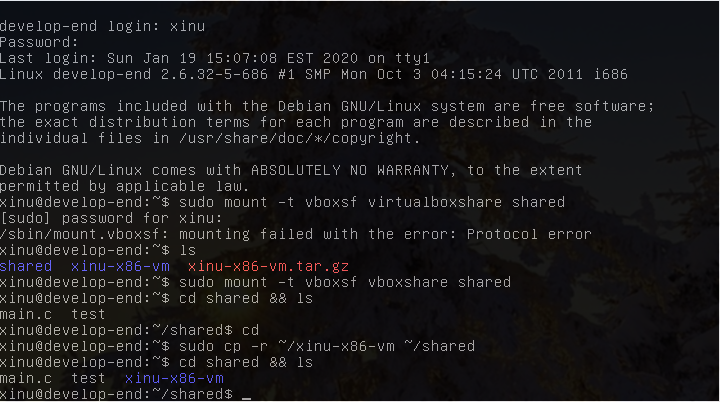
\includegraphics[width=\textwidth]{cp.png}
  \caption{Full command to copy directory.}
\end{figure}
\begin{figure}[ht!]
  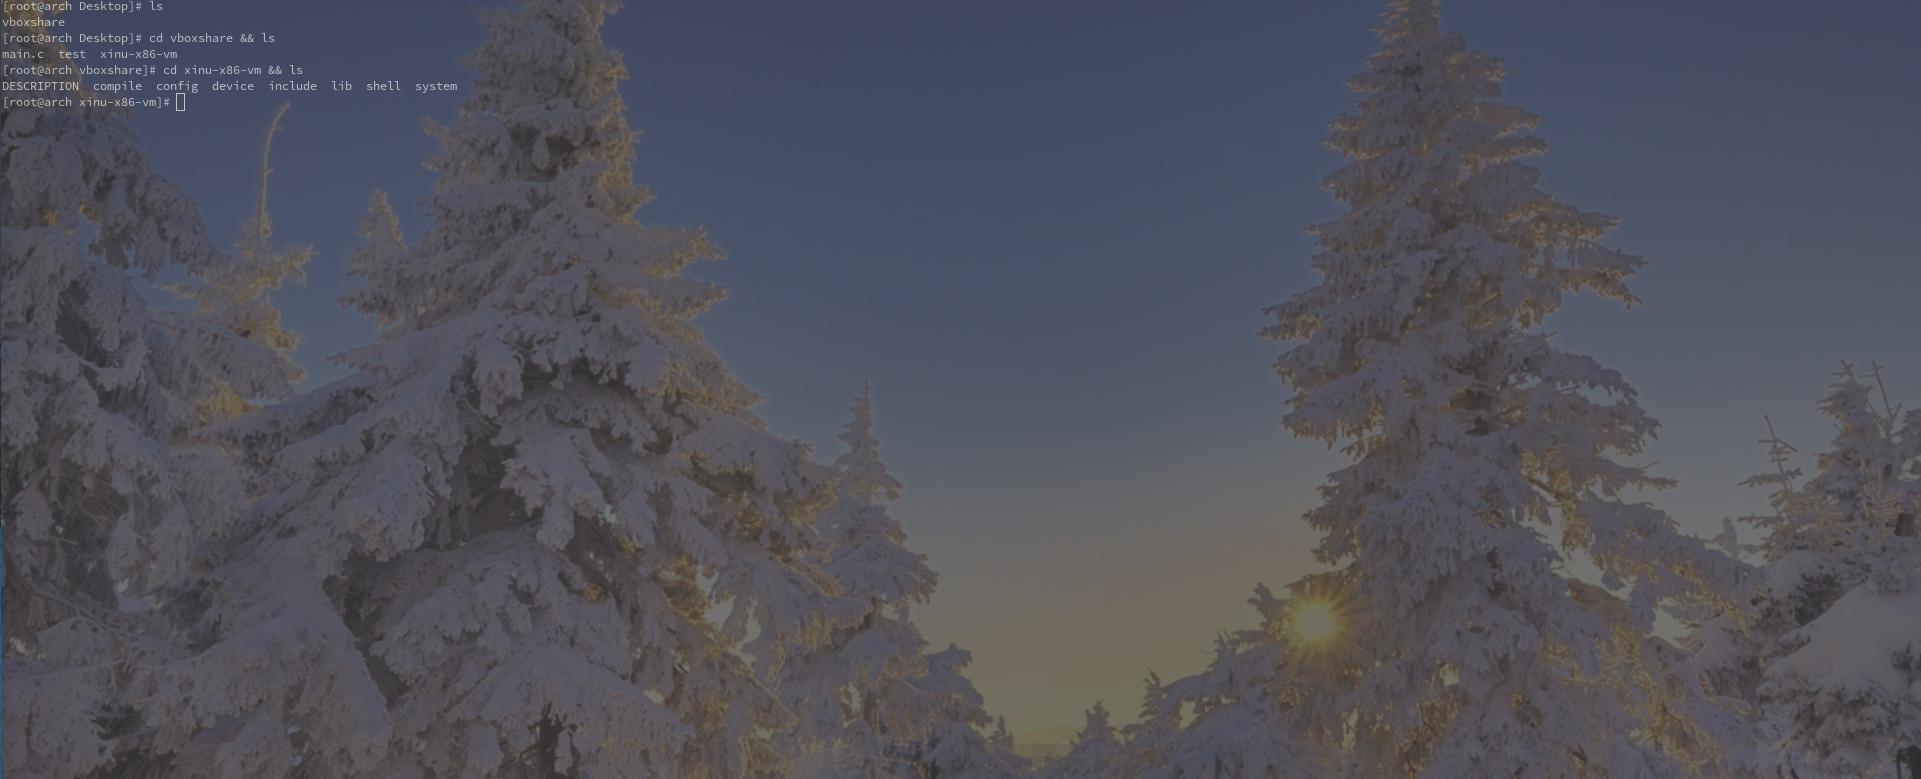
\includegraphics[width=\textwidth]{cp_home.png}
  \caption{My host computer, showing the contents of the shared directory.}
\end{figure}
\end{theorem}
\begin{theorem}
After I made a copy of of the "xinu-x68-vm" direcotry, I was able to recompile the "upload.sh" script, and see the 
Xinu logo once again:
\begin{figure}[ht!]
  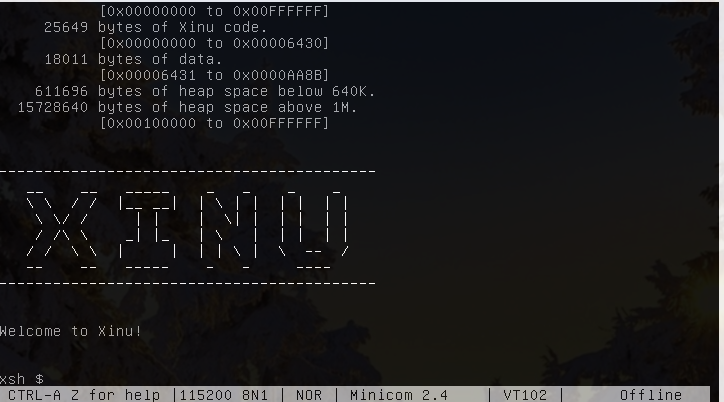
\includegraphics[width=\textwidth]{xinu2.png}
  \caption{Successful Xinu logo.}
\end{figure}
\end{theorem}

\section{Part III}
To edit "main.c", I chose to simply edit it using Vi within Xinu. I have a copy of the entire directory 
stored on my host computer, so just in case I needed
that code again, I would have it. To further protect myself, I just added the required text above the orginal "main.c"
in the file, with block quotes around it (using /* and */):
\begin{figure}[ht!]
  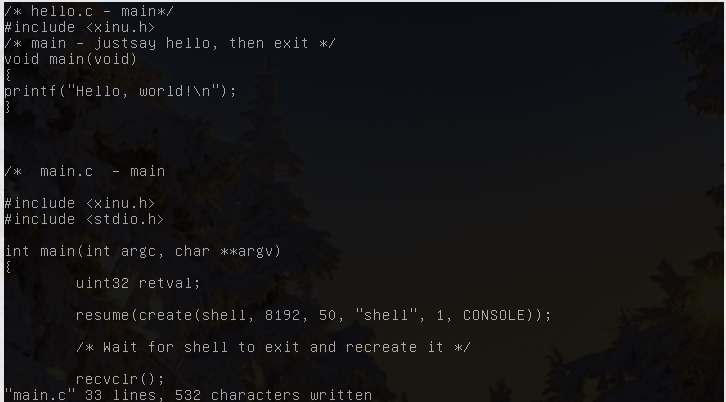
\includegraphics[width=\textwidth]{mainmod.png}
  \caption{Main.c edited with Vi, in Xinu.}
\end{figure}
\begin{figure}[ht!]
  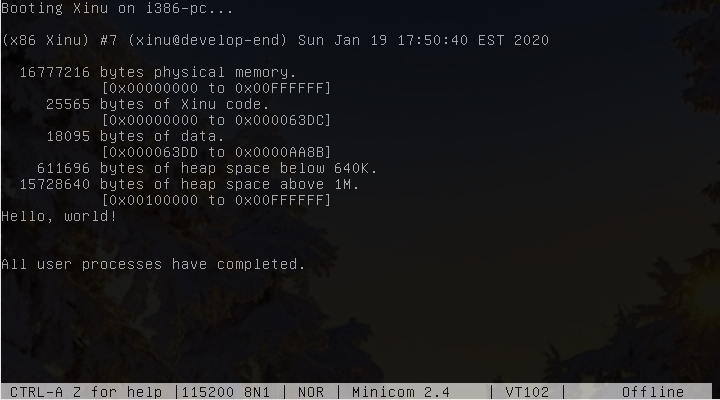
\includegraphics[width=\textwidth]{mainhello.png}
  \caption{Successful "Hello, world!" after restarting the minicom.}
\end{figure}

\section{Part IV}
\begin{theorem}
To edit "main.c" this time, I used the copy on my host machine (while keeping the original function commented out). My Vim text
editor has error checking for C built in, so it was easier for me to check for errors before compiling. After saving on 
my host machine, I copied the file out of the shared directory and into the system directory, and the recompiled:
\begin{figure}[ht!]
  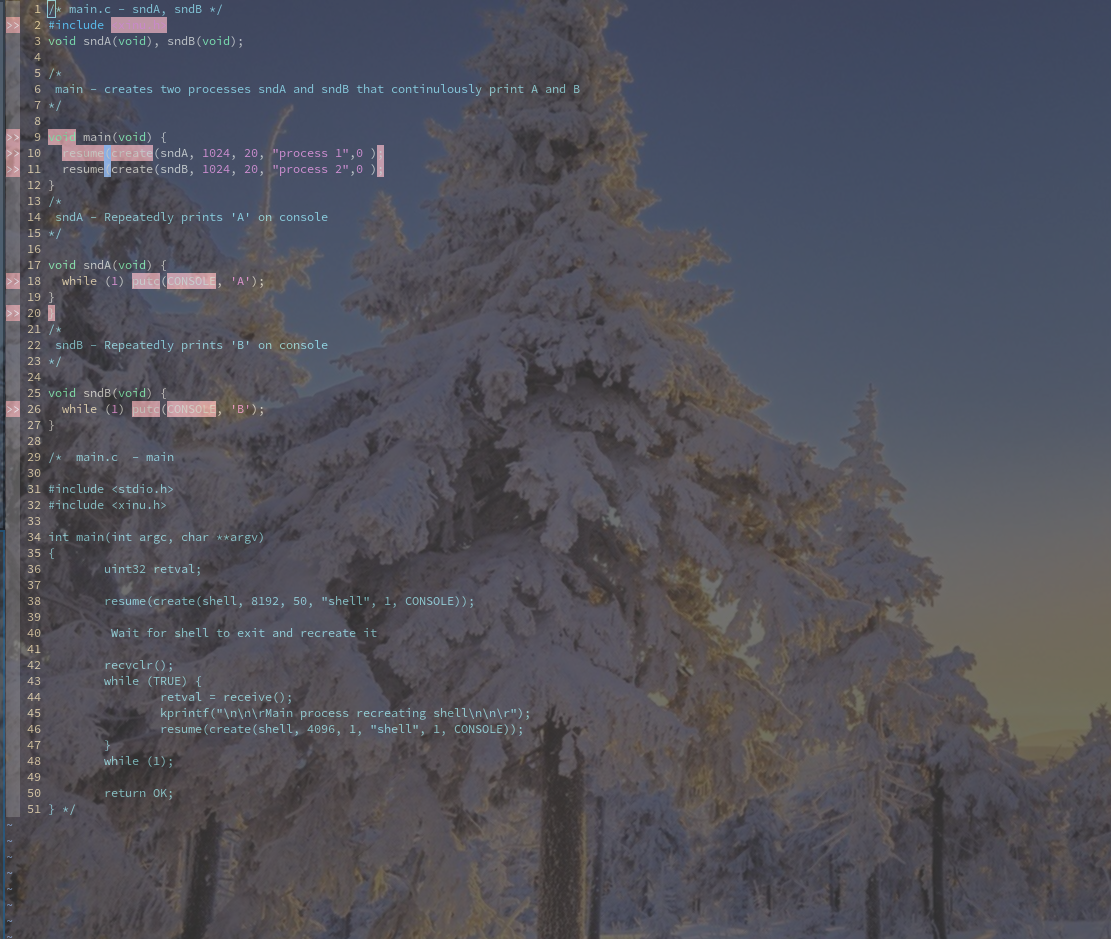
\includegraphics[width=\textwidth]{mainmod2.png}
  \caption{Main.c edited with Vim on my host machine.}
\end{figure}
\begin{figure}[ht!]
  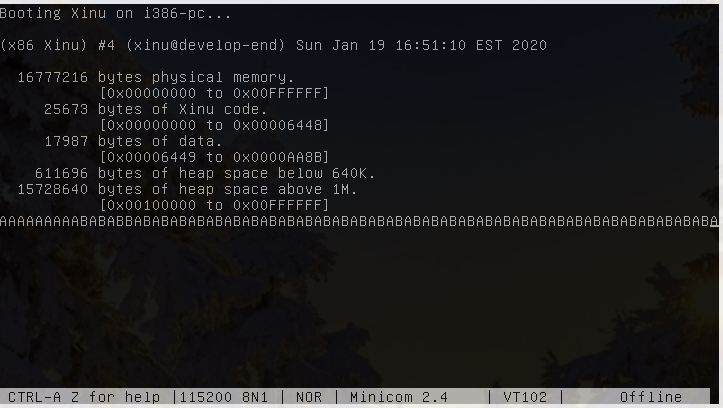
\includegraphics[width=\textwidth]{mainout.png}
  \caption{Output of newly modified main.c.}
\end{figure}
\end{theorem}

\section{Part V}
\begin{theorem}
After witnessing the relatively similar output of As to Bs, I assume changing the priortiy of sndA from 20 to 40 would
make the program print more Bs. My guess is the lower number (i.e. closer to 1), the higher the priority.
\end{theorem}

\begin{theorem}
I modified the main.c file direclty in Xinu again, changing the priority of sndA to 40. The result is almost completely As:
\begin{figure}[ht!]
  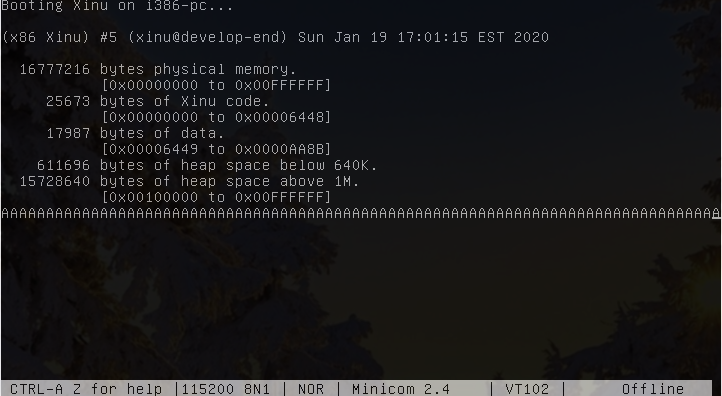
\includegraphics[width=\textwidth]{mainout2.png}
  \caption{Output with newly changed priority.}
\end{figure}\\\\
I believe the reason there are actually more As than Bs is because the higher priority number means more weighting is given
to that task's priority. Upon thinking about it further, I could see this being useful as new processes are added: if a more
important process is created and we need to assign higher priority, we can simply use the max of the current highest, and 
increment from there.
\end{theorem}
\end{document}
